\section{Sistemas Distribuídos}

    Tanenbaum e Steen no livro \textit{Sistemas Distribuídos: Princípios e Paradigmas} define um sistema distribuído como: %(Andrew S. Tanenbaum; Maarten Van Steen. “Sistemas Distribuídos: Princípios E Paradigmas.” 2ª ed. Prentice Hall Brasil: São Paulo – SP, 2007.)

    \begin{quote}
        ``Um conjunto de computadores independentes que se apresenta a seus usuários como um sistema único e coerente.''
     \end{quote}

    Dessa maneira tem-se que um sistema distribuído é composto por diferentes computadores autônomos que se comunicam entre si através de uma rede, dando ao usuário a sensação de que está em um sistema único. Tendo em vista que cada nó desse sistema é um computador independente, esse tipo de sistema permite que ele seja extremamente escalável, basta adicionar ou retirar uma instância para que esse sistema cresça ou diminua. A comunicação entre os nós desse sistema deve ocorrer de forma oculta ao usuário, fazendo com que ele não perceba que está lidando com diferentes computadores. Os sistemas distribuídos também ajudam na disponibilização contínua dos serviços, pois mesmo que algumas partes estejam temporariamente indisponíveis o sistema deve continuar funcionando sem que o usuário perceba quais são essas partes comprometidas.

    Essa sensação de estar em um único sistema é devido a uma camada de software intermediária que os sistemas distribuídos costumam possuir, que é situada logicamente entre uma camada de nível mais alto (usuários e aplicações) e uma camada de nível mais baixo (sistemas operacionais e protocolos de comunicação), por esse motivo, essa camada é chamada de middleware.

    A Figura \ref{fig:sistema-distribuido} representa um sistema distribuído com quatro computadores em rede permitindo que os componentes de uma aplicação se comuniquem com eles mesmos e ao mesmo tempo se comuniquem com diferentes aplicações. Os sistemas operacionais utilizados em cada máquina não necessariamente é o mesmo, porém o middleware faz uma camada de abstração que traz a sensação ao usuário de estar em um sistema único.
            
    % \begin{figure}[h]
    %         \centering
    %         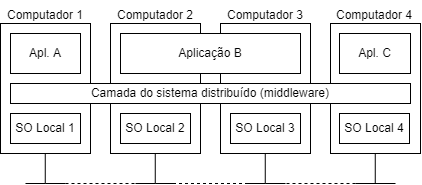
\includegraphics[scale=0.6]{figuras/sistema-distribuido.png}
    %         \caption{Sistema distribuído organizado como middleware - Imagem retirada de \cite{}.}
    %         \label{fig:sistema-distribuido}
    % \end{figure}

    % FIGURA
    % Figura 1 – Sistema distribuído organizado como middleware - Imagem retirada de (Andrew S. Tanenbaum; Maarten Van Steen. “Sistemas Distribuídos: Princípios E Paradigmas.” 2ª ed. Prentice Hall Brasil: São Paulo – SP, 2007.)


    